\documentclass[14Q,twocolumn]{jsarticle}
\usepackage[dvipdfmx]{graphicx}
\usepackage{wrapfig}
\usepackage{float}
\usepackage{otf}
\usepackage{longtable}
\usepackage{ulem}
\usepackage{ascmac}
\usepackage{multicol}
%%%%%
\makeatletter
\newenvironment{tablehere}
  {\def\@captype{table}}
  {}
\newenvironment{figurehere}
  {\def\@captype{figure}}
  {}
\makeatother
%%%%%%
\setlength{\textwidth}{160truemm}      % テキスト幅: 160mm
\setlength{\fullwidth}{\textwidth}     % ページ全体の幅
\setlength{\oddsidemargin}{0mm}   % 左余白
\setlength{\topmargin}{-10mm}       % 上余白
\setlength{\textheight}{240truemm}     % テキスト高さ: 297-(30+30)=237mm
\pagestyle{empty}
\title{ラスタ地図を美しく表現する}% 文書のタイトル
\date{2018年9月18日}
\author{厚沢部町 石 井 淳 平}              % 著者

%------------------------------
\begin{document}
\maketitle
%\begin{multicols}{2}
\section{この時間に覚えること}
\begin{itemize}
\item DEMデータの表示を変更する。
\item DEMデータから新たな地形指標(ここでは陰影図)を作成する。
\item DEMデータと陰影図を重ねて陰影つきの段彩図を表示する。
\end{itemize}

%%%%
\section{ラスタデータの特徴}
\begin{itemize}
\item 正体は画像ファイル(TIFF形式が一般的)
\item 連続量(標高や傾斜量)が基本ですが、土地分類図や植生図のような離散量を扱うこともあります。
\item 標高や傾斜、植生など異なる指標を組み合わせた演算を行うことができます\footnote{
ラスタデータのメリット・デメリットとして「素早く描画できる」や「境界線を表現するには不向き」などの視覚表現要素が上げられる場合がありますが、ベクタとラスタの選択はそのような視覚表現を主たる要因として選ばれるわけではなく、どのような統計的な処理を行うのかによって決まります。野生動物の出没地点や土地分類図などは通常ベクタデータで保持されますが、選好分析などを行う場合にはラスタ化して処理を行うこともあります。
}。
\end{itemize}

%%%%
\section{段彩図を作成する}
\begin{enumerate}
\item 「レンダータイプ」のドロップリストから「単バンド疑似カラー」を選択します。
\item 「新規カラーマップを作成」の下にあるドロップリストから好きなカラーマップを選びます。
\item 「モード」を「等間隔」に変更します。
\item 「分類数」はデフォルトは5になっていますので、まずはこれで試します。
\item 「色の補完」は「離散的」を選ぶ。
\end{enumerate}

\begin{figurehere}
\centering
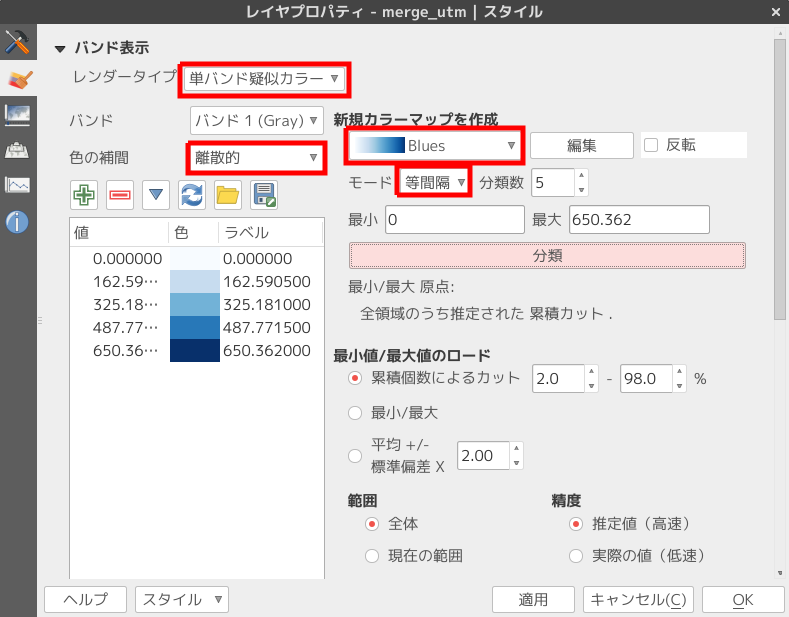
\includegraphics[width=1\linewidth]{03.png}
\caption{段彩図の作成}
\end{figurehere}

\begin{figurehere}
\centering
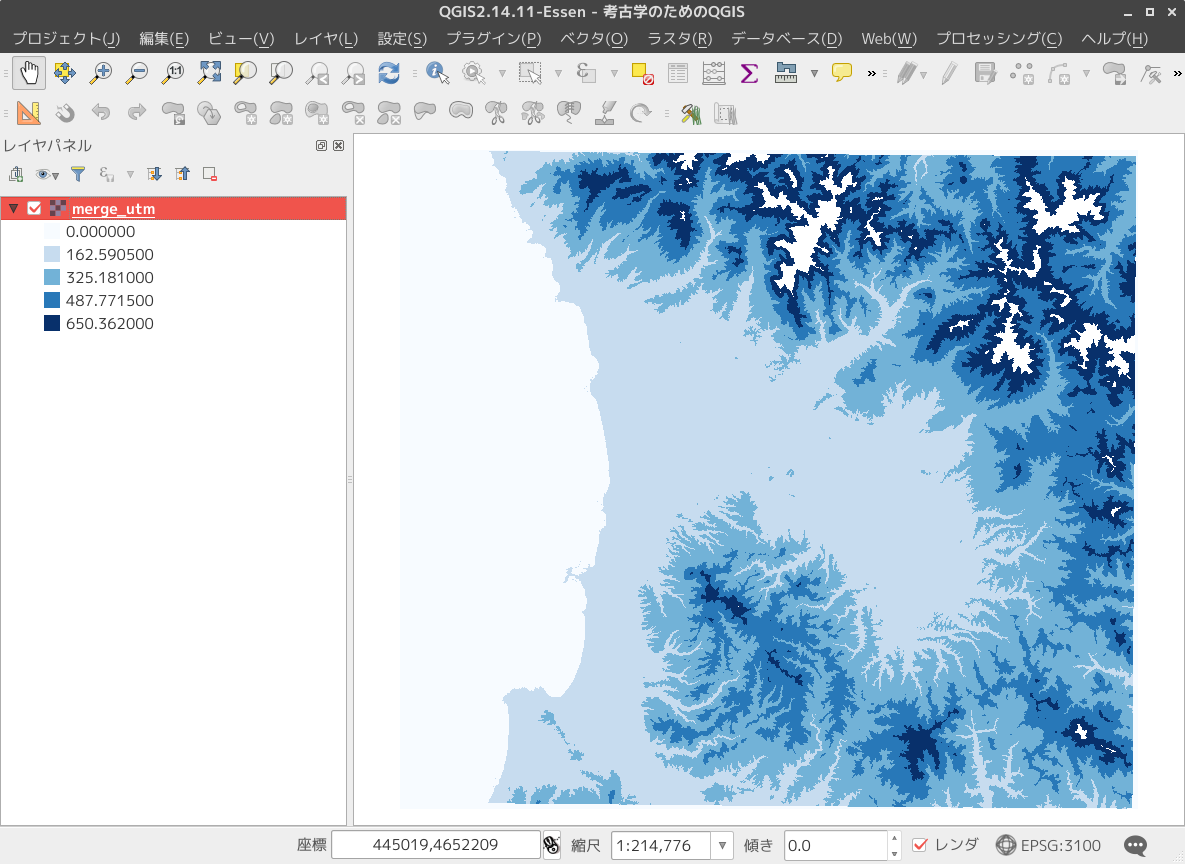
\includegraphics[width=1\linewidth]{05.png}
\caption{5段階で標高を区分した段彩図}
\end{figurehere}


%%%%
\section{陰影図を作成する}
\begin{enumerate}
\item 「ラスタ」→「地形解析」→「陰影図」
\item 「標高レイヤ」はDEMデータを指定します。この場合は「merge\_utm」です。
\item 「出力レイヤ」は新たに作成される陰影図の保存先を指定します。
\item 「出力形式」はデフォルトの「GeoTIFF」
\item 「Zファクタ」はデフォルトの「2」
\item 「イルミネーション」もデフォルトのままです。
\end{enumerate}

\begin{figurehere}
\centering
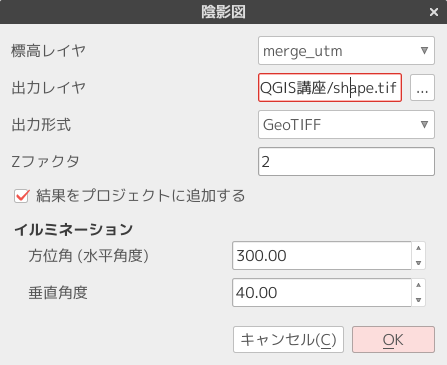
\includegraphics[width=0.8\linewidth]{08.png}
\caption{陰影図の作成}
\end{figurehere}

\begin{figurehere}
\centering
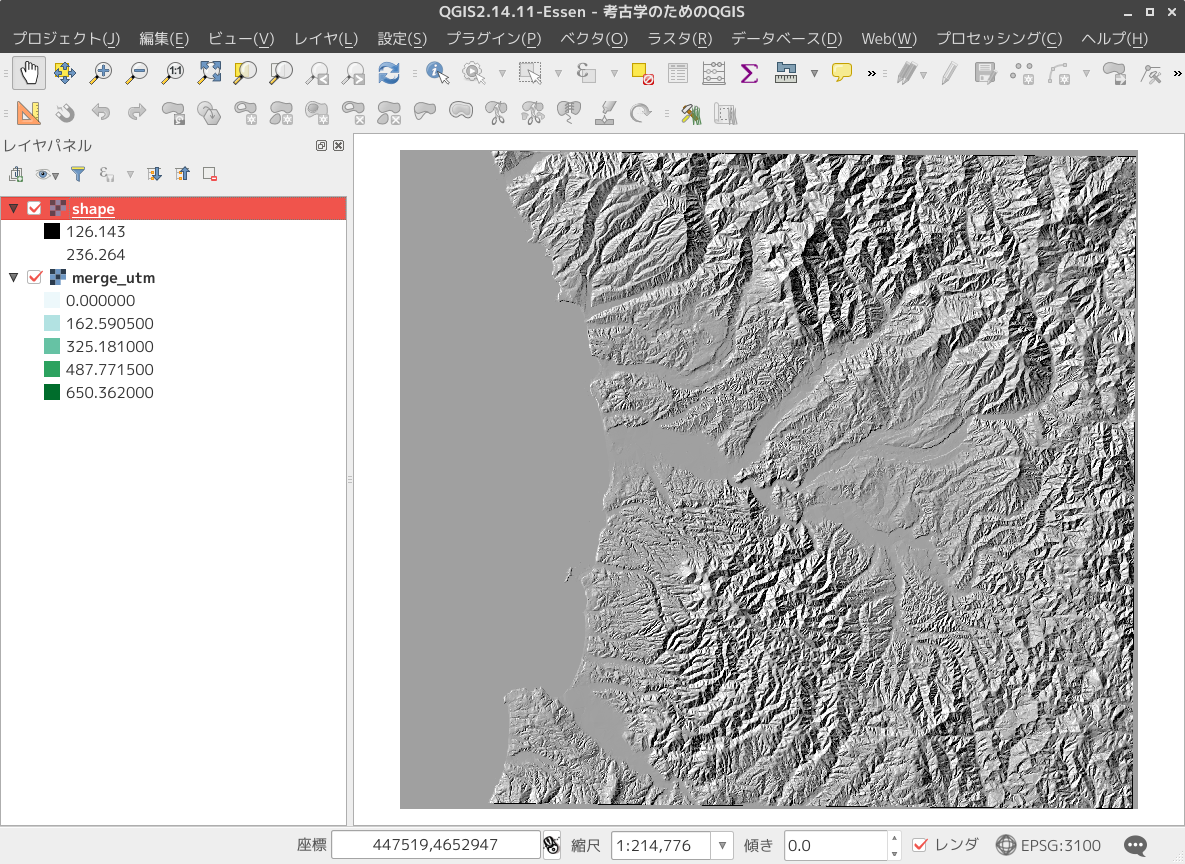
\includegraphics[width=1\linewidth]{09.png}
\caption{陰影図}
\end{figurehere}


%%%%
\section{透過率を変える}
\begin{enumerate}
\item 陰影図のレイヤ(Shapeレイヤ)を段彩図レイヤより上にします。
\item 陰影図レイヤをダブクリックして、レイヤプロパティを開きます。
\item 左側のタブの上から3番目の「透過性」タブを開きます。
\item  「全体の透過率」のスライダーを調整します。ここでは70\%に設定
\item 透過率は70\%〜80\%の間がもっとも適切に感じます。
\end{enumerate}

\begin{figurehere}
\centering
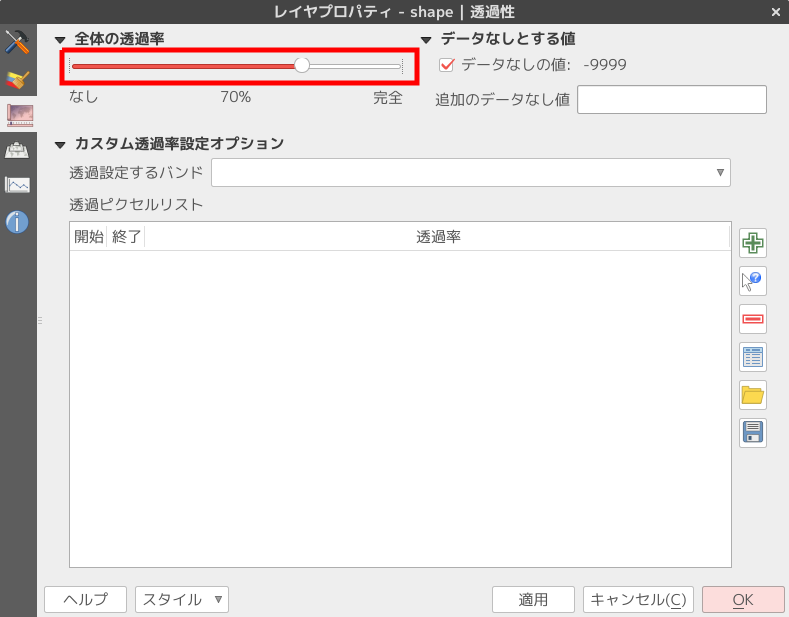
\includegraphics[width=0.8\linewidth]{10.png}
\caption{陰影図レイヤの透過率の変更}
\end{figurehere}

\begin{figurehere}
\centering
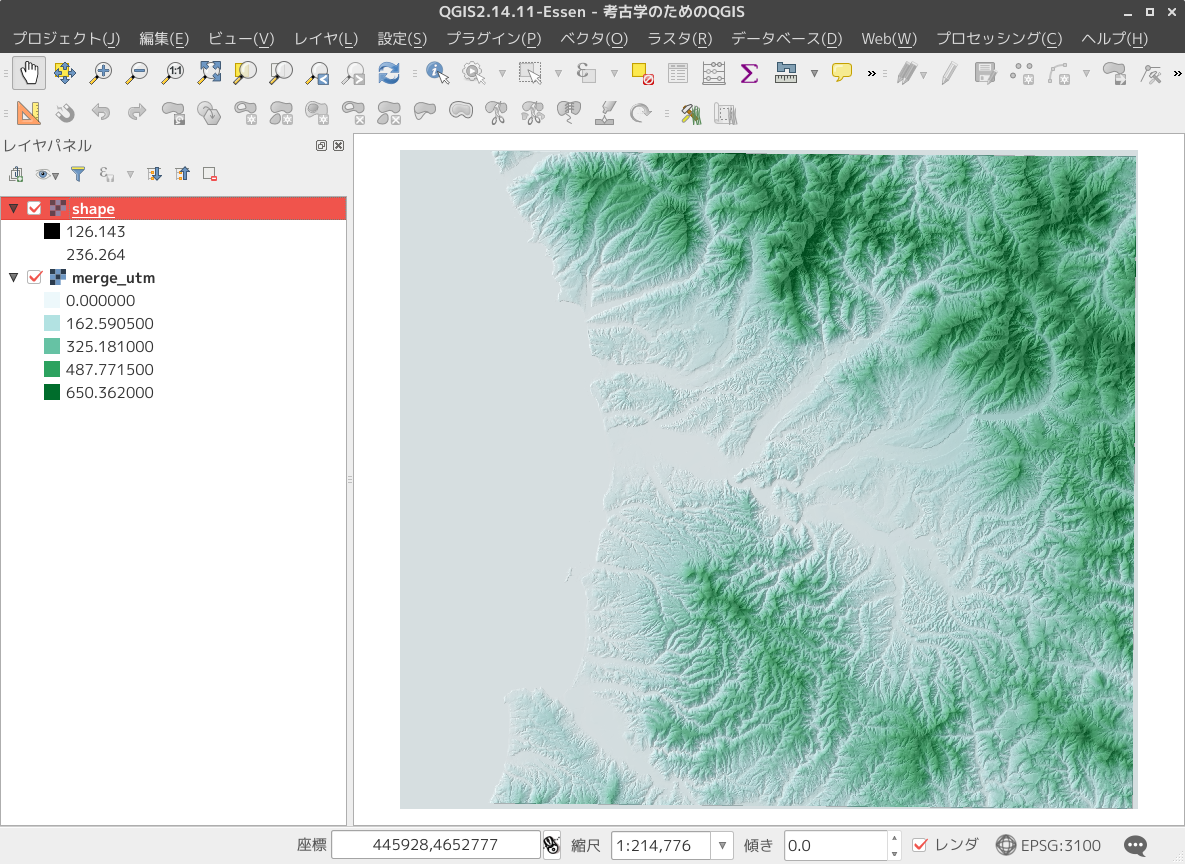
\includegraphics[width=1\linewidth]{11.png}
\caption{透過率を変えた陰影つき段彩図}
\end{figurehere}

\section{乗算で重ね合わせ}
\begin{enumerate}
\item 左側のタブの上から2番目の「スタイル」タブを開きます。
\item 下の方にある「カラーレンダリング」の「混合モード」を「乗算」に設定します。
\end{enumerate}

\begin{figurehere}
\centering
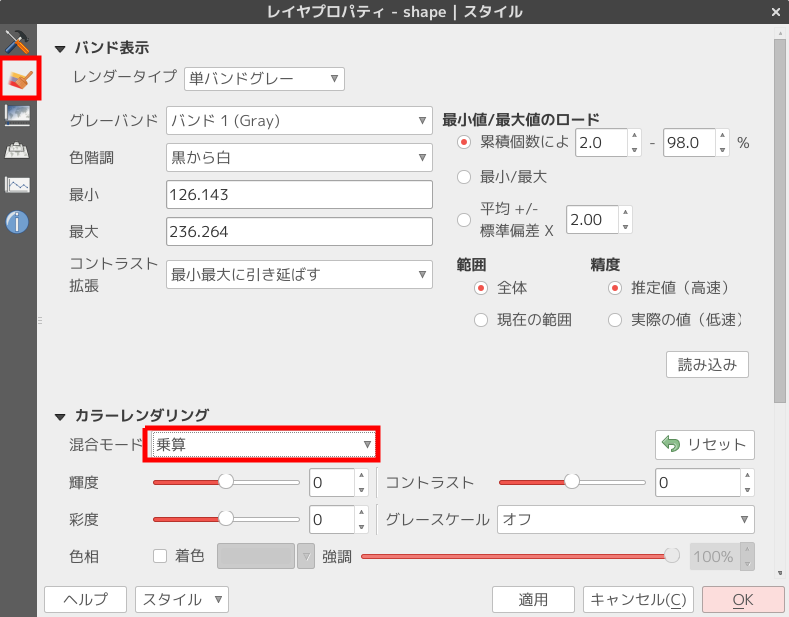
\includegraphics[width=0.8\linewidth]{13.png}
\caption{混合モードを「乗算」に変更}
\end{figurehere}

\begin{figurehere}
\centering
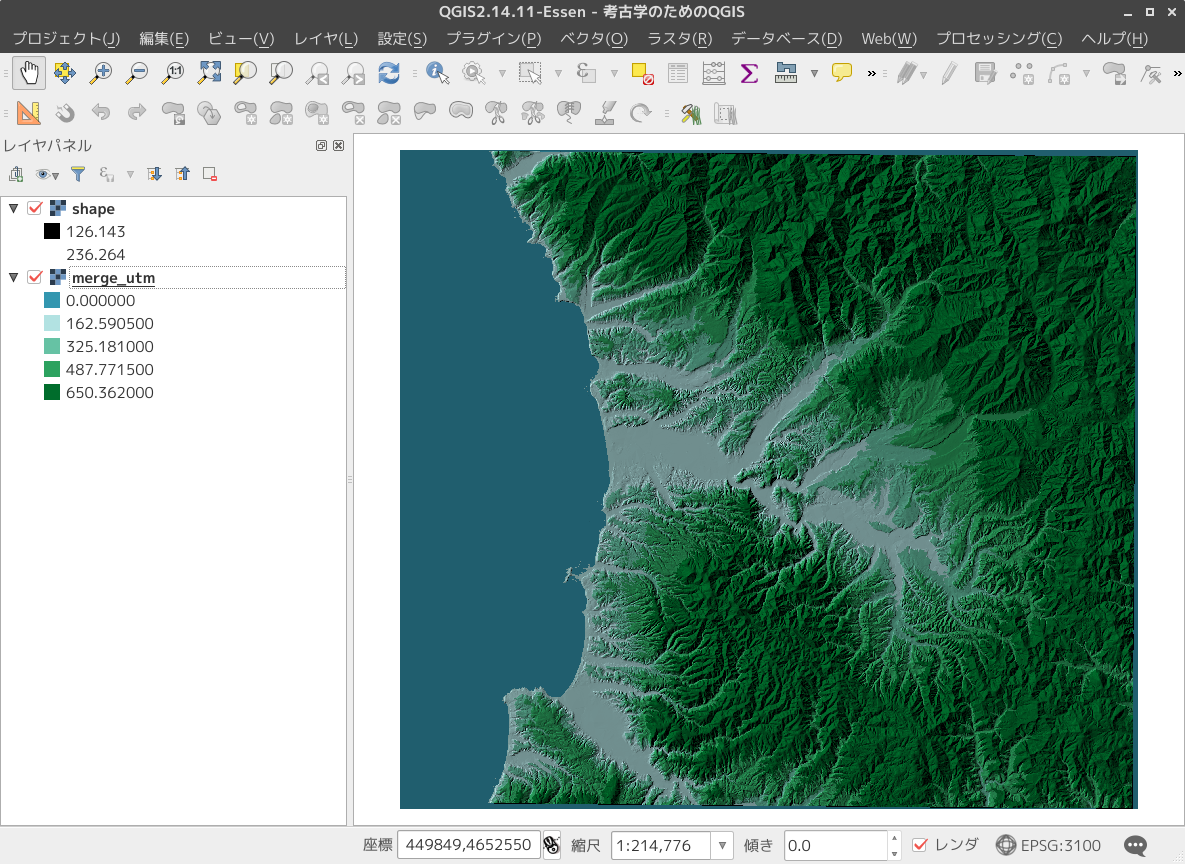
\includegraphics[width=1\linewidth]{15.png}
\caption{乗算による陰影つき段彩図}
\end{figurehere}

\begin{figurehere}
\centering
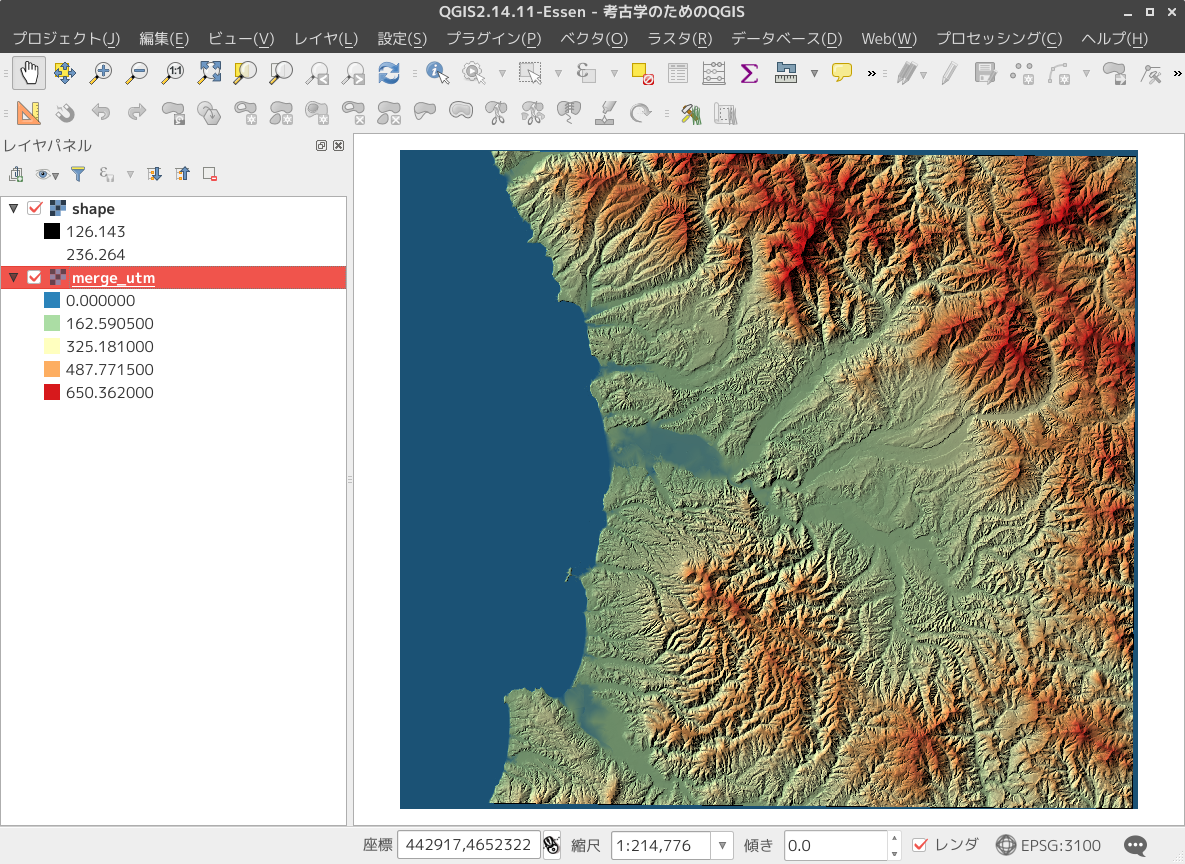
\includegraphics[width=1\linewidth]{16.png}
\caption{表現を変えた段彩図}
\end{figurehere}


%\end{multicols}
\end{document}
